\title{Assignment 2.1}
\author{
        Pradyot Prakash - 130050008
            \\
        Utkarsh Mall - 130050037
			\\
		Samarth Mishra - 130260018
}
\date{\today}
\documentclass[11pt]{article}
\usepackage[left=2.5cm,top=2cm,right=2.5cm,bottom=2cm,bindingoffset=0.5cm]{geometry}
\usepackage{graphicx}
\usepackage{siunitx}
\graphicspath{ {../images/} }
\renewcommand\thesubsection{\Alph{subsection}}
\begin{document}
\maketitle

\subsection{myIntegration()}
Chosen step size $\Delta s = 1$. If a step size larger than this is chosen then information present image will missed as step size is larger than pixel size.
Choosing step size smaller than this is computationally expensive and the results of integration will be very similar to that of $\Delta s = 1$.

Bilateral interpolation is being used here. A Nearest Neighbour interpolation will not be a good estimate of integral compared to integral evaluated by bilinear interpolation.
In cases like $\Delta s = 0.66$ with integration along an axis,NN interpolation will select alternate pixels with twice(not a good estimate), which will not be the case with bilinear interpolation.
\subsection{myRadon()}

\begin{figure}[h]
\centering
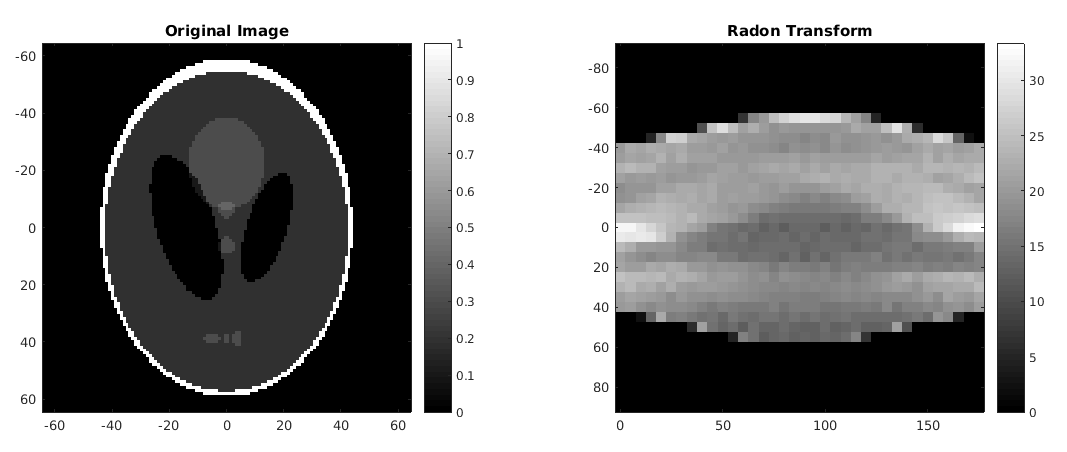
\includegraphics[scale=0.4]{b}
\caption{Shepp Logan Phantom Image and its Radon transform}
\end{figure}

\subsection{Parameter Choice}
The Radon Transform image with $\Delta s=1$ and $\Delta s=0.5$ look smoother than the transform with $\Delta s=3$. 
However there is no significant difference in images with $\Delta s=1$ and $\Delta s=0.5$(Figure 2).

The Radon Transform along a single $\theta$ with $\Delta s=1$ and $\Delta s=0.5$ are very similar and are smoother than the transform with $\Delta s=3$ (Figure 3).

In case of $\Delta s=3$ we are skipping over pixels while integrating, because of which a small change in parameter on integration line can result in big changes in integral hence smalled $\Delta s$ gives smoother function as well as image.

\begin{figure}[h]
\centering
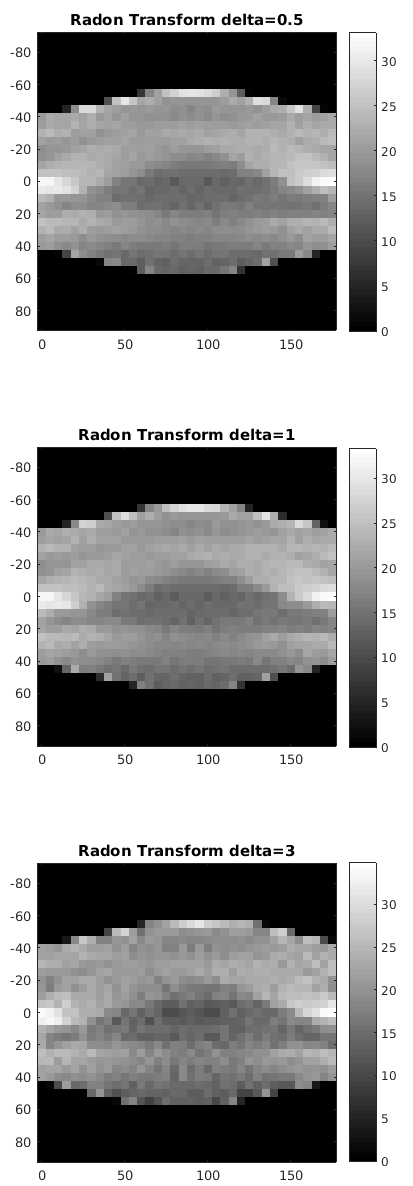
\includegraphics[scale=0.45]{c}
\caption{Shepp-Logan Phantom Image's Radon transform with $\Delta s = 0.5,1,3$ respectively}
\end{figure}
\begin{figure}[h]
\centering
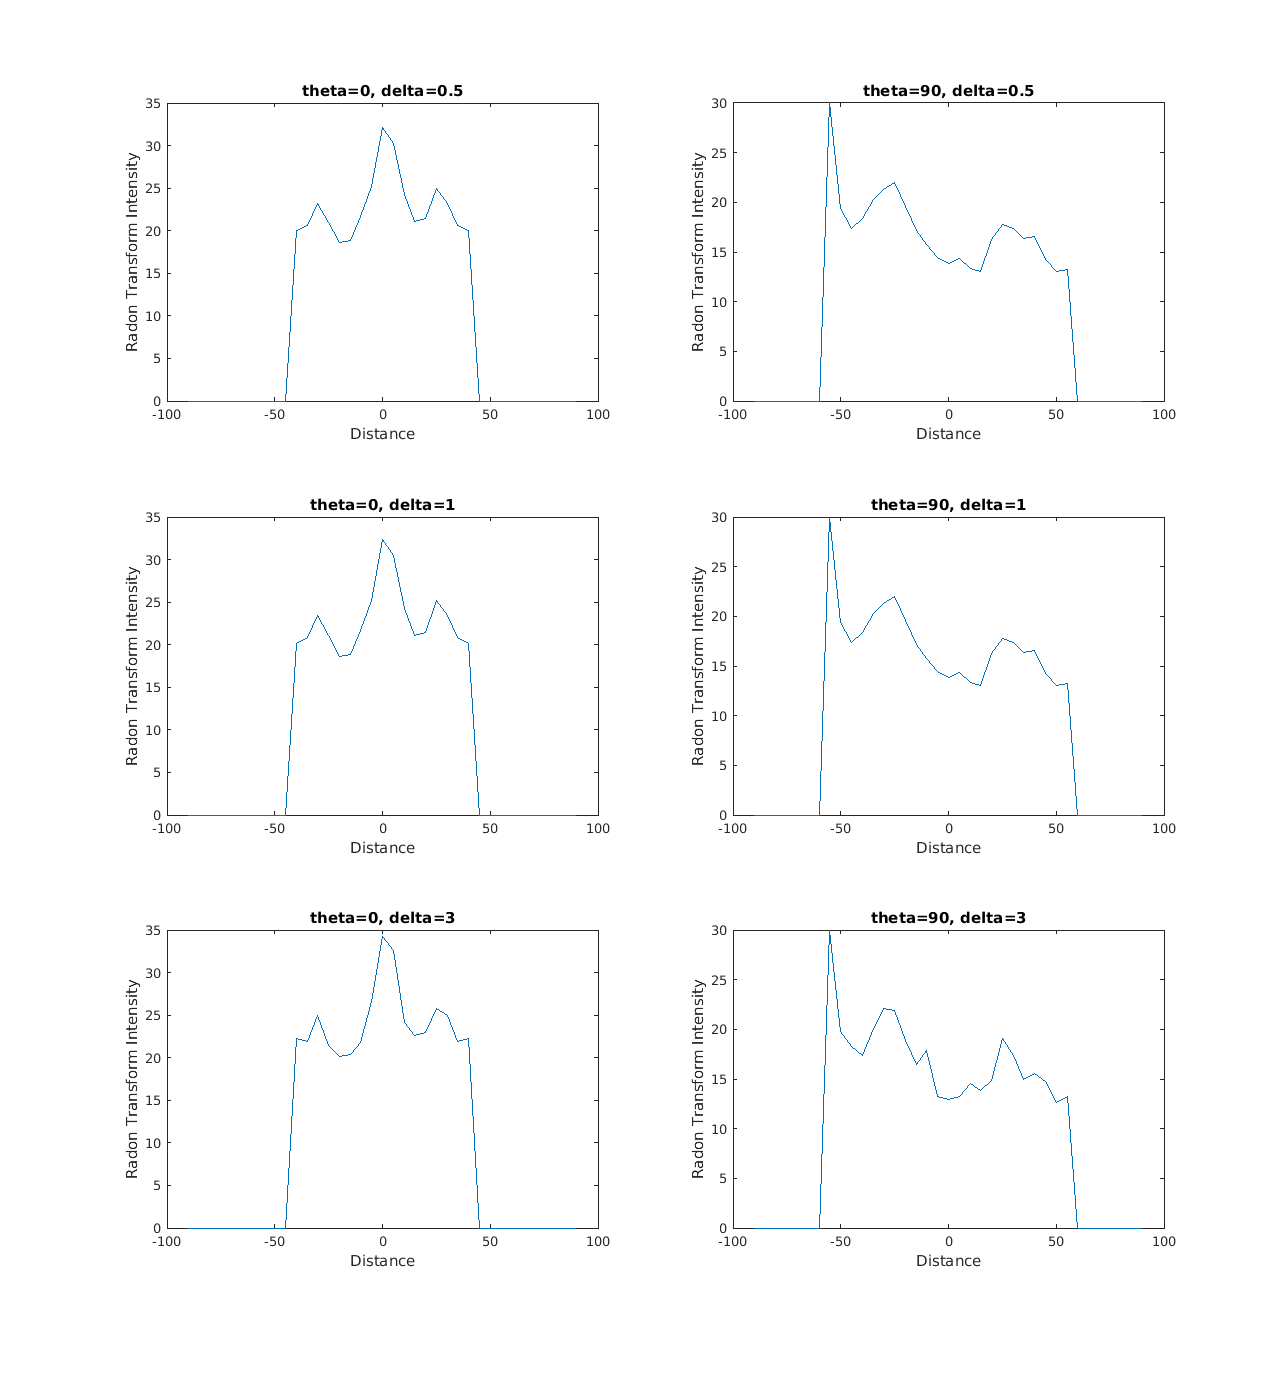
\includegraphics[scale=0.4]{c2}
\caption{Shepp-Logan Phantom Image's Radon transform Intesity along $\theta=0^{0} $ and $\theta=90^{0} $ with $\Delta s = 0.5,1,3$ respectively}
\end{figure}

\subsection{$\Delta t$ and $\Delta \theta$}
Smaller $\Delta t$ and $\Delta \theta$ the transform will be able to capture more fine details. However, Since transforms are applied on a discrete domain very small $\Delta t$ and $\Delta \theta$ will have minimal effect on accuracy of transform, also it will be computationally expensive.

\subsection{Algebraic Reconstruction Technique}

\end{document}
